a

\section{Introduction}


Video inpainting aims to recover the missing content of a corrupted video and assist lots of practical applications,~\emph{e.g.,} video restoration and watermarking removal. 
High-quality video inpainting requires not only realistic structures with visual details but also temporal consistency. 
%Compared with image inpainting, video inpainting is significantly more challenging due to the extra time dimension, while human eyes are sensitive to flickers and jitters.
% 
Though great progress has been made in 2D image inpainting using deep learning techniques \cite{yu2018free,Xiong_2019_CVPR}, directly applying these approaches to each frame individually for video inpainting will lead to flaws, flickers, and jitters due to the additional time dimension. 

\begin{figure}[t]
	\centering
	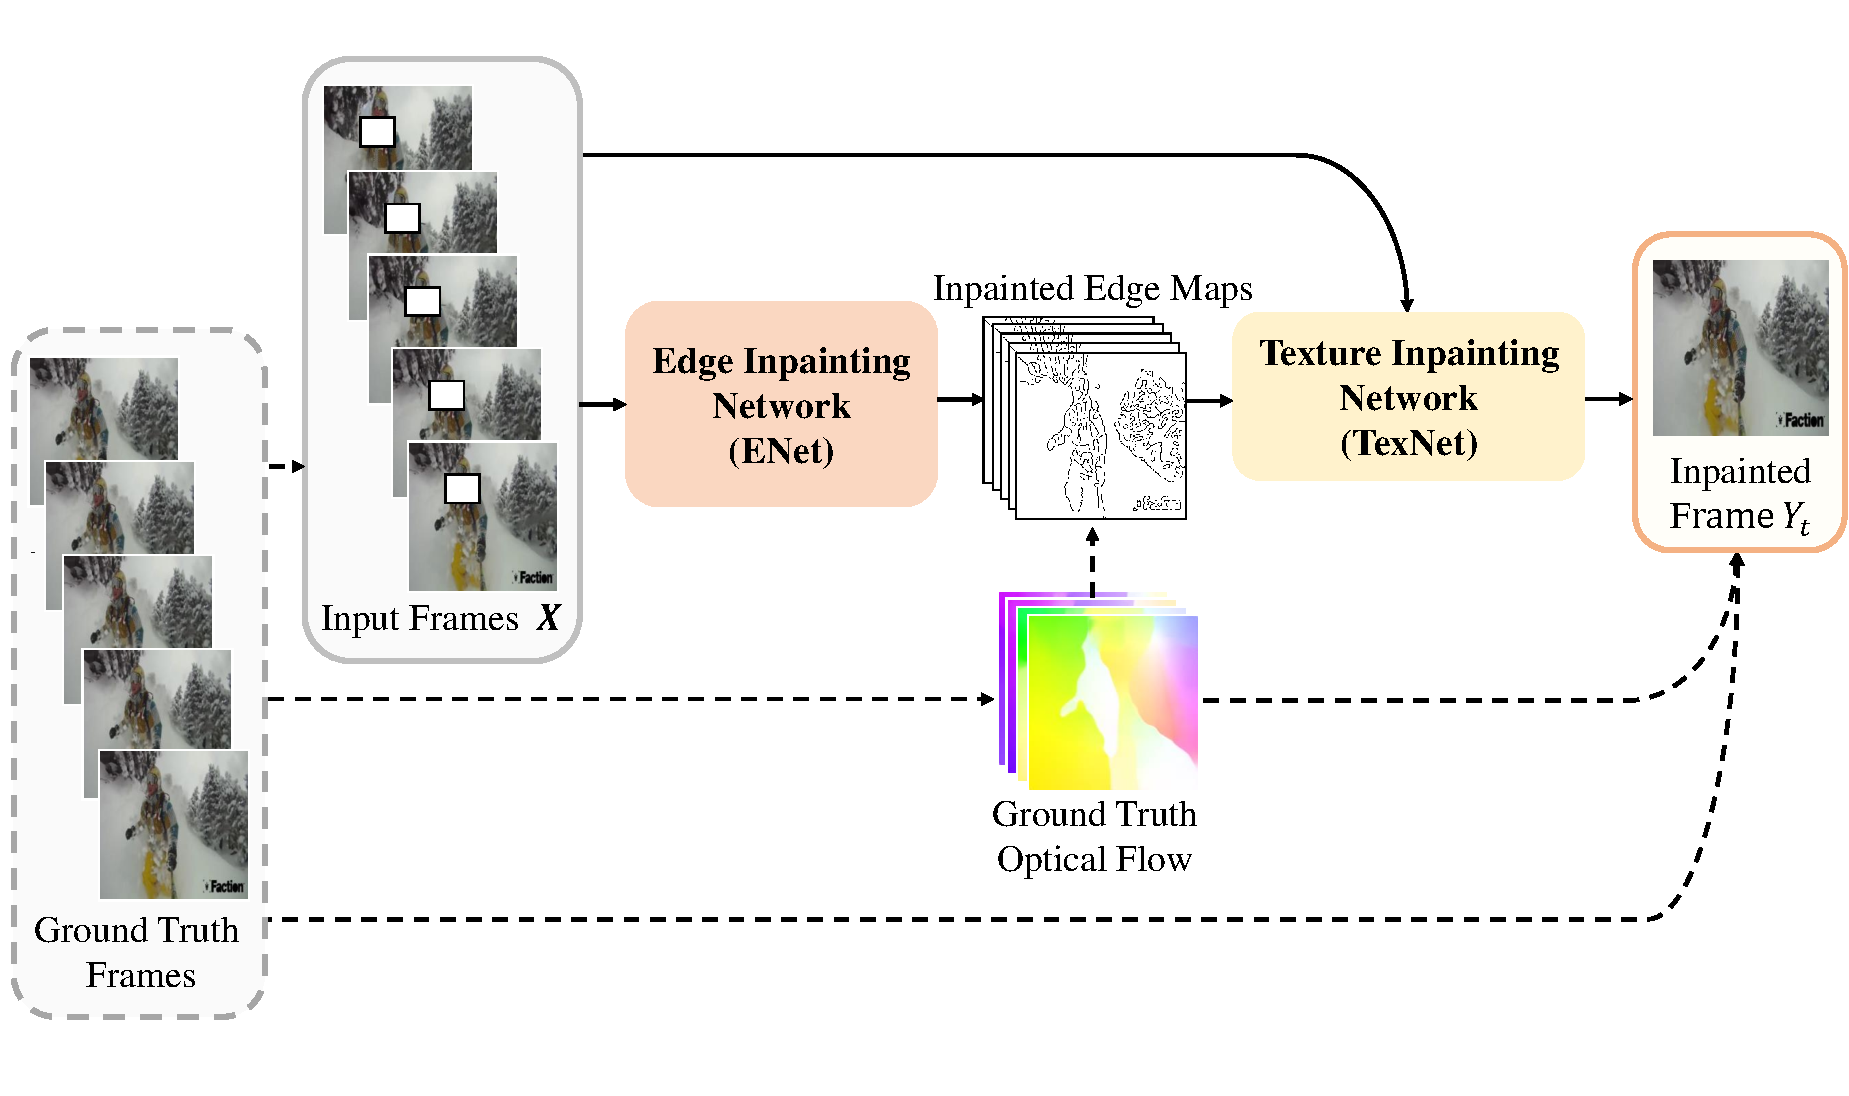
\includegraphics[width=1.01\columnwidth]{zong} % Reduce the figure size so that it is slightly narrower than the column. Don't use precise values for figure width.This setup will avoid overfull boxes. 
	\caption{Overview of our structure-guided inpainting network. We first complete the missing edges by aggregating information from neighboring frames to represent the target structure using the ENet. Then, the TexNet synthesizes the missing textures under the guidance of structure edges. Besides, the ground truth optical flow is utilized during the training stages of both ENet and TexNet to enforce temporal coherence, which is denoted by dotted lines.}
	\label{zong}
\end{figure}



\begin{figure*}[!t]
	\centering
	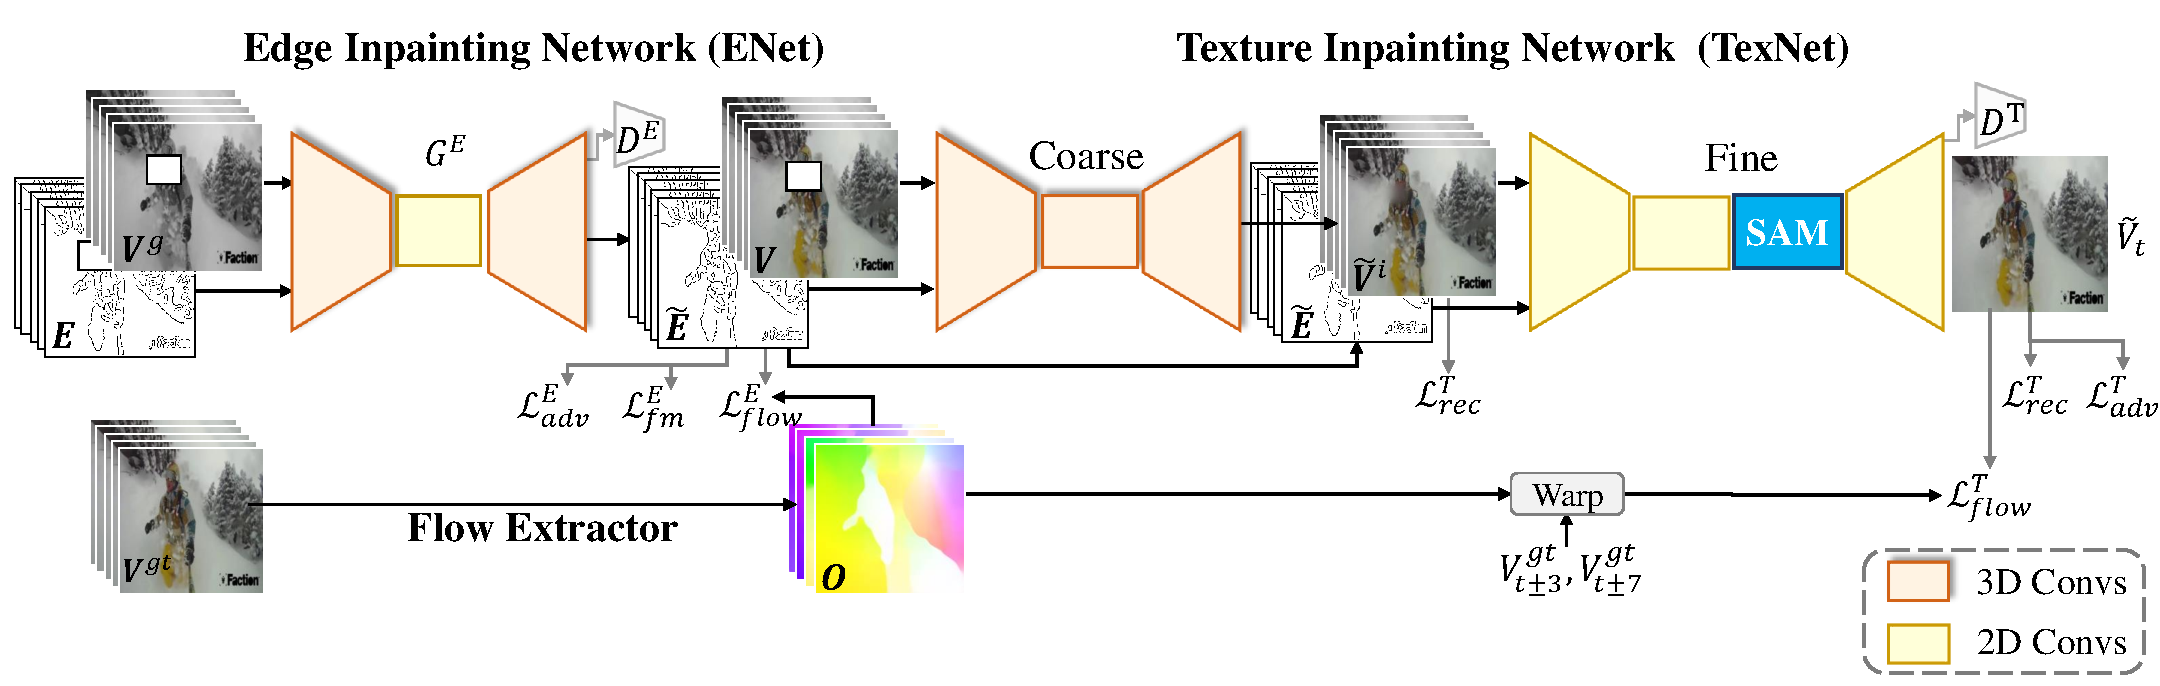
\includegraphics[width=2.05\columnwidth]{sti} % Reduce the figure size so that it is slightly narrower than the column. Don't use precise values for figure width.This setup will avoid overfull boxes. 
	\caption{The detailed architecture of our network. ENet adopts an encoder-decoder architecture to complete edges in the missing regions. TexNet utilizes a coarse-to-fine manner to inpaint the final frames. Ground truth optical flow between adjacent frames are extracted for edge consistency loss and frame warping loss. }
	%FNet is based on the backbone Resnet-101, which is associated with ENet.
	
	\label{fig:stiNet}
\end{figure*}




Traditional video inpainting methods employ a patch composition framework by exploiting complementary information across neighboring frames and compositing visually pleasing content in the missing regions via patches~\cite{patwardhan2007video,wexler2004space,newson2014video}.
% 
These methods rely heavily on the hypothesis that the missing content in the corrupted region appears in neighboring frames, which greatly limits their generalization ability.
%
Recently, deep-learning-based methods achieve great performance improvement in video inpainting.
A straightforward solution is to utilize 3D convolution layers to extract spatio-temporal features and predict missing content with smooth motion \cite{wang2019video}.
To obtain temporally smooth results, optical flow is commonly used by aggregating contextual information from neighboring frames~\cite{Kim_2019_CVPR1,Xu_2019_CVPR,Kim_2019_CVPR}.
For example, a deep optical flow completion network is proposed to propagate missing pixels across frames~\cite{Xu_2019_CVPR}. 
Kim~\emph{et al.} leverage recurrent feedback to utilize potential information in previous frames~\cite{Kim_2019_CVPR,Kim_2019_CVPR1}.
By introducing motion guidance, these methods pay more attention to temporal smoothness; however, structure rationality and object details have not been well explored. 
%However, structural rationality is also a significant factor for realistic video inpainting. 
%
Without definite representation and generation of the target image structures, these methods tend to produce over-smoothed regions. 
Similar observations have been obtained in image inpainting \cite{Xiong_2019_CVPR,nazeri2019edgeconnect}.
%\cite{iizuka2017globally,liu2018partialinpainting,yu2018free}. 
To solve this problem, two-step methods have been proposed to complete object contours~\cite{Xiong_2019_CVPR} or edge maps~\cite{nazeri2019edgeconnect} first as auxiliary information to guide texture synthesis in image inpainting later.
%
However, when applying these edge-first image inpainting methods to video inpainting, it brings another challenge in generating temporally coherent structures when human vision is significantly sensitive to temporal discontinuity that frequently occurs at edges. 


In order to simultaneously hallucinate detailed image structures and preserve temporal coherence in video inpainting, we present a novel structure-guided video inpainting approach which effectively exploits the spatio-temporal structure information to improve the quality of video inpainting.  
%
Compared with previous video inpainting methods that only consider the motion information, we explore the correlation among structure, motion, and texture to complete the missing region with reasonable structure, rich visual details, and temporal coherence, as shown in Fig.~\ref{fig:..}.
% first, edge -- structure
First, we design an EdgeNet to predict sparse edges in the missing region that represent the target structure information for each frame by exploiting the spatio-temporal neighboring information from adjacent frames.
%Second, texture
Then, under the guidance of completed edges, TexNet fills the textures via a coarse-to-fine architecture and a structure attention module (SAM).
Specifically, the SAM is designed to guide the texture generation of TexNet by capturing the latent spatial relevance between video textures and completed structure edges.
Notably, such a structure-texture relevance can effectively improve the fine-detailed frame generation in TexNet with less cracks and better object contours.
%Then we fill textures under the guidance of concise edges.
%Third, motion
To enhance the temporal coherence of synthesized frames, we employ motion flows for consistency check of both edge maps and inpainted frames during the training stage.
%
The ground truth optical flow is exploited to guide both ENet and TexNet to generate temporal smooth edge maps and texture results via edge consistency and frame warping constraints.
% are respectively utilized to align the edge maps and final inpainted texture between frames. 
Consequently, the inpainted frames using our approach are not only temporally consistent, but also completed in structure and rich in visual details.
The detailed comparison between the proposed method and related state-of-the-art methods is given in Table~\ref{tab:comparison}.



\begin{table}[t]
\begin{center}
\caption{Detailed comparison between our method and related state-of-the-art methods. Our method utilizes both auxiliary temporal optimization (Flow) and spatial optimization (Edge), which guarantees spatio-temporal coherence explicitly.} \label{tab:comparison}
%\resizebox{1\columnwidth}{!}{
\begin{tabular}{c|c|c|c}
  \hline
  \multirow{2}{*}{}&Temporal&Spatial&Explicit Spatio-Temporal\\
  &Opt.&Opt.& Coherence\\
  \hline
  \hline
 Edge-Connect \cite{nazeri2019edgeconnect} &\xmark &Edge& \xmark    \\
  \hline
  CombCN \cite{wang2019video} & \xmark &\xmark &\xmark     \\
  \hline
  DVI \cite{Kim_2019_CVPR1} &  Flow    &\xmark & \xmark    \\
  \hline
  DFVI \cite{Xu_2019_CVPR} & Flow    &\xmark &\xmark               \\
  \hline
  Ours&Flow&Edge&\cmark\\
  \hline
\end{tabular}%}
\end{center}
%\vspace{-0.4cm}
\end{table}


%As shown in Fig.~\ref{zong}, our method mainly consists of two modules, which are respectively an edge inpainting network (ENet) and a texture inpainting network (TexNet).
% and flow guidance constraints (denoted by dotted lines).
%Given multiple adjacent frames with masks, ENet first completes edge maps that depict the target structure via a 3D+2D architecture. 



%In summary, we present a novel structure-guided video inpainting method, which can generate structural reasonable and temporal coherent inpainted frames.
%
Experiments on the YouTubeVOS and DAVIS datasets show that the proposed method obtains new state-of-the-art inpainting quality with low time consumption.
%
Our technical contributions can be summarized as follows:
\begin{itemize}
	\item We propose a novel structure-guided video inpainting method, which integrates scene structure, texture, and motion to complete the missing region with valid structure, rich visual details, and temporal coherence.
	% explore the correlation 	
	\item A structure attention module is designed to capture the correlation between structure edges and video textures, which can provide better structural guidance for texture synthesis. % edge - texture 
	\item A flow-guided edge warping loss and a frame warping loss are developed to enhance the temporal consistency of both completed edges and video frames.   
\end{itemize}


%The rest of this paper is organized as follows. Section~\ref{sec:rw} reviews the related works. Section~\ref{sec:approach} illustrates the proposed video inpainting method. Section~\ref{sec:exp} provides the experiments on YouTubeVOS and DAVIS datasets, and Section~\ref{sec:conclu} concludes the whole paper.





\section{Related Work}
%Our method are mostly related to (a) traditional image/video inpainting, (b) CNN-based image inpainting, and (c) deep video inpainting. We will introduce them in this section below.
Image or video inpainting has been studied for decades. 
%\paragraph{Traditional Image/Video Inpainting}
Traditional methods of image and video inpainting can be divided into two categories, diffusion-based and patch-based methods. 
Diffusion-based methods \cite{bertalmio2000image,ballester2001filling} gradually propagate contents from surrounding areas to the missing region. 
Li \emph{et al.}~\cite{li2017localization} attempt to solve the problem of localization of diffusion-based inpainted regions.
Li \emph{et al.}~\cite{li2016image} define diffusion coefficients according to the relation between the damaged pixel and neighborhood pixel.
Fractional-order nonlinear diffusion driven by difference curvature is proposed to produce more sharp object boundaries \cite{sridevi2019image}. 
However, this kind of method fails to handle large holes due to its assumption of local smoothness. 
%
Patch-based methods, also called exemplar-based methods ~\cite{bertalmio2003simultaneous,efros2001image}, are more widely studied.
They formulate the completion task as a patch-based optimization problem. 
Barnes \emph{et al.}~\cite{barnes2009patchmatch} employ approximate nearest neighbor algorithm to fill the damaged regions.
Sangeetha \emph{et al.}~\cite{sangeetha2011combined} propose to propagate both linear structure and two-dimensional texture into the target region.
Ru{\v{z}}i{\'c} \emph{et al.} \cite{ruvzic2014context} introduce Markov random field to help search the most matched candidates.
Ding \emph{et al.} \cite{ding_19nonlocal} employ nonlocal texture similarity and local intensity smoothness to produce natural-looking results.
Besides, some patch-based methods utilize low rank approximation. For example, Guo \emph{et al.} \cite{pb_lowrank2018} propose a simple two-stage low rank approximation to recover the corrupted region, which avoids time-consuming iterations.
Lu \emph{et al.} \cite{lu2018gradient} adopt gradient-based low rank approximation.
Patch-based \cxj{image?} methods fill the missing content by borrowing and aggregating the most similar patches based on low-level image features from known regions and pasting them to unknown parts. However, this type of method usually fails when there are insufficient information in known regions or image textures are too complicated.  
%

As for patch-based video inpainting, a series of methods have been proposed by searching patches across frames~\cite{patwardhan2007video}, extending the 2D PatchMatch algorithm~\cite{barnes2009patchmatch} to improve inpainting quality \cite{newson2014video}, or jointly estimating optical flow and textures to promote temporal coherence \cite{huang2016temporally}.
Y. Wexler \emph{et al.} \cite{wexler2007space} constrain masked regions to synthesize coherent structures with respect to reference examples based on local structures. 
Y. Umeda \emph{et al.} \cite{umeda2012removal} propose using directional median filter as complementation of patch-based filling.
Some methods separate foreground and background apart, and then deal with the two parts respectively with different algorithms, since there naturally exists property differences between them.  
A. Ghanbari \emph{et al.} \cite{ghanbari2011contour} first separate the two parts in videos, and fills the two parts accordingly with the help of contours.
A. Xia \emph{et al.} \cite{xia2011exemplar} make use of Gaussian mixture models to also distinguish moving foreground and still background, and process them separately.   
  
%However, traditional metshods assume that there exist similar contents in known regions, thus fail to synthesize unseen appearances. 
However, the propagation process makes these methods suffer from high computational complexity, which limits their usage in practical applications. 




\paragraph{CNN-based Image Inpainting}
Recently, deep learning methods have achieved  tremendous progress in the filed of computer vision, for example, image recognition \cite{krizhevsky2012imagenet,he2016deep}, object detection \cite{ren2015faster,redmon2016you}, and semantic segmentation \cite{long2015fully,chen2017deeplab}. 
The tasks of image and video inpainting also witness great promotion thanks to the capability of deep learning networks to capture high-level semantic information in images and videos.
%
The convolution neural network (CNN) is first introduced for image denoising and inpainting in \cite{xie2012image}, where CNN is used to directly synthesize image contents in the masked regions.
To improve the photorealism of the completed results, a generative adversarial network is employed \cite{pathak2016context}. 
Then, C. Yang \emph{et al.} \cite{yang2017high} takes advantages of multi-scale representation to boost details generation.
%by jointly training a generator and a discriminator in a minimax manner. 
Multiple discriminators are used to constrain both global and local coherence of image contents \cite{iizuka2017globally}.  
J. Yu \emph{et al.} \cite{yu2018generative} proposes the contextual attention module to capture long-range information.
Subsequent approaches solve more specific problems in image inpainting. For example, inpainting irregular holes with partial convolution~\cite{liu2018partialinpainting} and employing gated convolution \cite{yu2018free} for dynamic feature selection. Both these two method want to handle image inpainting with irregular regions, which is hard for vanilla convolutions. 
%
While these methods tend to generate over-smoothed and blurry results, a two-stage approach is proposed to hallucinate edges first and then fill image colors using the edges as a prior \cite{nazeri2019edgeconnect}. Similarly, W. Xiong \emph{et al.} \cite{Xiong_2019_CVPR} predict contours of foreground objects to guide the inpainting process of masked regions.
Though high-quality static images with reasonable structure can be generated using these methods, simply extending it from image to video by 3D convolutions inevitably fails because of no guarantee on the temporal coherence. Besides, these methods simply utilize edges and contours as one of the inputs of the image inpainting network, without the mechanism to utilize the structure information more efficiently. 
%These image inpainting methods can obtain plausible synthesized images. 
%\cite{nazeri2019edgeconnect} introduces an edge generator to refine generated structure in image inpainting. 


%%% video inpainting 
\paragraph{Deep Video Inpainting}
%However, directly extending these state-of-the-art image inpainting methods to video domain is not an optimal solution, which will generate videos with serious temporal flickers, artifacts, and jitters. 
Besides the challenge in maintaining temporal coherence, image inpainting methods do not fully utilize useful complementary information in neighboring frames, which could help large hole completion in videos.
Several methods regarding video inpainting based on deep neural networks have been proposed just recently.
%
The first deep-learning-based video inpainting method is CombCN \cite{wang2019video}, which jointly learns temporal structure and spatial details via 3D convolutions.
%%\cite{Xu_2019_CVPR} proposes a stacked convolution network to predict missing motion field and regards video inpainting as a pixel propagation problem. 
%
To enforce temporal coherence, a recurrent feedback is employed to connect consecutive frames~\cite{Kim_2019_CVPR,Kim_2019_CVPR1}. 
Instead of filling pixel colors directly using CNNs, a deep flow completion network is proposed to propagate pixel colors based on the estimated flow in the missing region~\cite{Xu_2019_CVPR}.
%However, these existing methods neglect the importance of intact structure in video inpainting and typically suffer from blurs and structural cracks in the synthesized frames.  
\mdf{However, these existing methods usually suffer from blurs and structural cracks in the synthesized frames since it is non trivial to maintain fine details and sharp edges when predicting temporally coherent pixel colors. }
%
In comparison, we propose to explicitly complete the target structure using edges, which are efficient to predict due to their sparsity. To utilize the information more effectively, we introduce a structure attention mechanism. 
Under the structural guidance, more pleasing results could be synthesized with reasonable structure and fine details. 

%Different from the methods above, we extract and refine structure information explicitly, which will generate fine-detailed video inpainting results.

%\cite{Kim_2019_CVPR} automatically removes texts in videos without mask indications, which aggregates temporal features from encoder to decoder and applies a recurrent feedback. 
%\cite{Kim_2019_CVPR1} introduces convolutional LSTM and temporal feature aggregation to obtain temporal consistency and learn information from neighboring frames. 




























